\documentclass{article}
\usepackage[]{url}
\usepackage{graphicx}
\usepackage{hyperref}
\usepackage{mathtools}
\usepackage{tikz}
\usepackage{subcaption}

\begin{document}
\title{Collective motion of squirmers in confined environments}
\author{Roth Robin\\
\\
Supervisors: Van Landeghem Céline, Giraldi Laetitia,\\ Agathe Chouippe}
\date{May, 2024}
\maketitle

\tableofcontents

\section{Introduction}
This internship is the continuation of a project realised during the year. The main goal of the project was
to develop numerical methods for driving micro-robots composed of magnetic heads and flexible tails imitating spermatozoa, reffered to as squirmers.\\
A python code has been implemented during the project, it simulates the behaviors of two interacting squirmers by computing 
the forces and torques present.\\
\section{Context}
The collective behavior of active particles is well studied in the literature. 
The Vicsek model is frequently used to model these active particles. 
The aim of this internship is to perform a similar study considering squirmers, 
in various confined domains and to compare the collective motion of the squirmers with that of the active particles using the Vicsek model. 
The motion of the squirmers is simulated using two different models: a continuous model that approximates hydrodynamic and 
steric forces, and a full model using the finite element library Feel++.

\section{Objectives}
The main goal is to model the dynamics of a schoal of squirmers within confined environments, 

\section{Vicsek}
\subsection{Model}
\begin{center}
    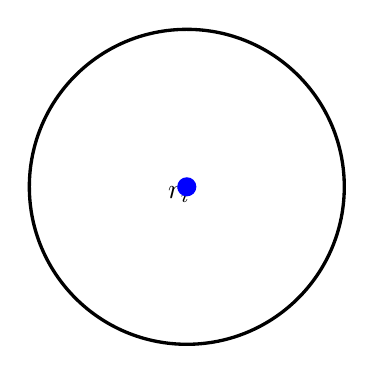
\begin{tikzpicture}
        \draw[color=black, very thick](0,0) circle (2);
        \node at (-0.1,-0.1) {{$r_i$}};
        \filldraw[color=blue, fill=blue, very thick](0,0) circle(0.1);
    \end{tikzpicture}
\end{center}
The Vicsek model consists of $N$ particles with $r_i(t)$ and $\theta_i(t)$ 
their position, velocity and orientation.\\
All particles have the same velocity $v_0$.
The evolution of the orientation $\theta_i(t)$ at each time step $\nabla t$ is:
$$\theta_i(t + \nabla t) = \langle\theta_j(t)\rangle_{|r_i(t) - r_j(t)| < R} + \epsilon_i(t)$$
with
$$\langle\theta_j(t)\rangle = \arctan\left(\frac{\sin(\theta_j(t))}{\cos(\theta_j(t))}\right)$$
$R$ the range of interaction, $\langle\theta_j(t)\rangle_{|r_i(t) - r_j(t)| < R}$ the average 
orientation of the particles in the range $R$ of
 the $i$-the particle (including itself) at the time $t$ and $\epsilon_i(t)$ represents the noise, 
 it's a random number taken from a uniform probability distribution
over $\left(-\frac{\eta}{2}, \frac{\eta}{2}\right)$.\\
The parameter $\eta$ is the main tool that counteracts the alignment of the particles.\\
\\
The evolution of the position $r_i(t)$ at each time step $\nabla t$ is:
$$ r_i(t + \nabla t) = r_i(t) + v_0\nabla t \begin{pmatrix}
    \cos(\theta_i(t))\\
    \sin(\theta_i(t))
\end{pmatrix}$$
The velocity is described by $\vec{v}_i(t)$ which is defined by
$$\vec{v}_i(t) = v_0\begin{pmatrix}
    \cos\theta_i(t)\\
    \sin\theta_i(t)
\end{pmatrix}$$
The behavior of the particles are quantified by the polar order parameter $v_a$ which is calculated with:
$$v_a = \frac{1}{Nv_0}\left|\sum^{N}_{i=1}\vec{v}_i\right|$$

\subsection{Implementation}
\end{document}